\documentclass[12pt]{article}
\setlength\parindent{0pt}
\usepackage{fullpage}
\usepackage{amsmath}
\usepackage{graphicx}
\setlength{\parskip}{4mm}
%\usepackage[left=2cm, right=2cm, top=1.5cm, bottom=1cm]{geometry}
\usepackage[margin=0.5in, paperwidth=13.5in, paperheight=8.4375in]{geometry}
\def\LL{\left\langle}   % left angle bracket
\def\RR{\right\rangle}  % right angle bracket
\def\LP{\left(}         % left parenthesis
\def\RP{\right)}        % right parenthesis
\def\LB{\left\{}        % left curly bracket
\def\RB{\right\}}       % right curly bracket
\def\PAR#1#2{ {{\partial #1}\over{\partial #2}} }
\def\PARTWO#1#2{ {{\partial^2 #1}\over{\partial #2}^2} }
\def\PARTWOMIX#1#2#3{ {{\partial^2 #1}\over{\partial #2 \partial #3}} }
\newcommand{\BI}{\begin{itemize}}
\newcommand{\EI}{\end{itemize}}
\newcommand{\BE}{\begin{displaymath}}
\newcommand{\EE}{\end{displaymath}}
\newcommand{\BNE}{\begin{equation}}
\newcommand{\ENE}{\end{equation}}
\newcommand{\BEA}{\begin{eqnarray}}
\newcommand{\EEA}{\nonumber\end{eqnarray}}
\newcommand{\EL}{\nonumber\\}
\newcommand{\la}[1]{\label{#1}}
\newcommand{\ie}{{\em i.e.\ }}
\newcommand{\eg}{{\em e.\,g.\ }}
\newcommand{\cf}{cf.\ }
\newcommand{\etc}{etc.\ }
\newcommand{\Tr}{{\rm tr}}
\newcommand{\etal}{{\it et al.}}
\newcommand{\OL}[1]{\overline{#1}\ } % overline
\newcommand{\OLL}[1]{\overline{\overline{#1}}\ } % double overline
\newcommand{\OON}{\frac{1}{N}} % "one over N"
\newcommand{\OOX}[1]{\frac{1}{#1}} % "one over X"

\def\BS{\bigskip}

\begin{document}
\pagenumbering{gobble}
\Large
\centerline{\sc{Recitation Questions -- 1D Motion (part 2)}}
\normalsize
\centerline{\sc{16 February}}

\it You will be assessed in this recitation by a member of the teaching staff who will stop by for a brief conversation. Anyone participating in learning physics will get full credit; you don't need to do anything special.

\rmfamily

\medskip

\rm In this recitation, you will practice:

\BI
\item Translating back and forth between words and mathematics as a way to describe motion
\item Solving problems symbolically rather than numerically
\item Dealing with situations with a changing acceleration (piecewise constant)
\item Relating position, velocity, and acceleration graphically
\EI
\newpage


\centerline{\Large Question 1: a braking car}


A car is traveling at 30 m/s and applies its brakes to slow down to 10 m/s. If it is able to decelerate at 5 $\rm m/\rm s^2$, how far does it travel during the braking period?

\begin{enumerate}
\item Write expressions for the car's position and velocity as a function of time. What moment makes sense to choose as your reference time $t=0$?

\vspace{1in}


\item How can you translate the question ``How far does it travel during the braking period?'' into a sentence about your algebraic variables? Again, fill in the blanks: 

\begin{center}
{\bf ``What is the value of \underline{\hspace{0.7in}} at the time when \underline{\hspace{0.7in}} is equal to \underline{\hspace{0.7in}}?''} 
\end{center}


\item What intermediate quantity must you find before you find the distance traveled? Following the above recipe you created for yourself, find it.




\vspace{2in}





\item Finally, how far does the car travel during the braking period?



\end{enumerate}

\vspace*{\fill}
\begin{center}
\bf (If your group didn't finish this problem last week, do it here.) 
\end{center}

\newpage

\centerline{\Large Question 2: a braking car, with variables}

A car is traveling at a speed $v_0$ and applies its brakes to slow down to a speed $v_f$. If it is able to decelerate at an acceleration $a_b$, how far does it travel during the braking period?

\begin{enumerate}
\item Write expressions for the car's position and velocity as a function of time, as before.

\vspace{1in}


\item Using the same process that you did in the previous problem, find an expression that tells how far the car travels during the braking period. This should depend only on $v_0$, $v_f$, and $a_b$ -- the physical parameters of the problem. 

\vspace{3in}

\end{enumerate}
\newpage

\centerline{\Large Question 3: a rocket}
\begin{minipage}{0.3\textwidth}
A small rocket is pointed straight up and fired. Its motor burns for $\tau=10$ s; while the rocket's motor burns, it
accelerates upward at $a_r=15 \rm m/\rm s^2$; after it burns out, the rocket is in freefall. (To make the numbers simpler for 
this problem, and for every problem in this class, you may use $g=10\, \rm m/\rm s^2$.)


Before you do any mathematics, sketch graphs on the rest of this page for the rocket's acceleration vs. time, velocity vs. time, and position vs. time, in that order, from the time the rocket leaves the ground to when it returns to the ground. (Here I've labeled the height $y$ rather than $x$ since it is moving vertically.) Remember:

\BI
\item The slope of the velocity graph should be equal to the value of the acceleration graph, since acceleration is the derivative of velocity
\item The slope of the position graph should be equal to the value of the velocity graph.
\EI

This means that:

\BI
\item When the acceleration is positive, the velocity should be increasing, and the position should be concave up;
\item When the acceleration is negative, the velocity should be decreasing, and the position should be concave down;
\item When the velocity is zero, the position graph should have a maximum or minimum
\EI

\end{minipage}
\begin{minipage}{0.75\textwidth}
\begin{center}
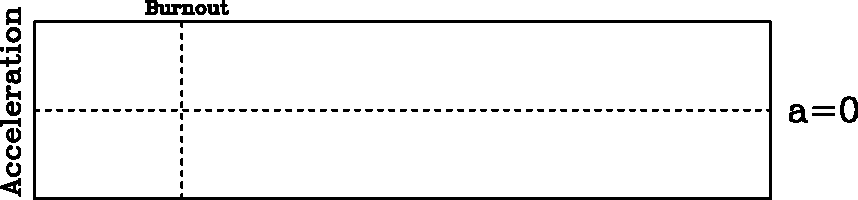
\includegraphics[width=0.85\textwidth]{avst-plain-crop.pdf}\\
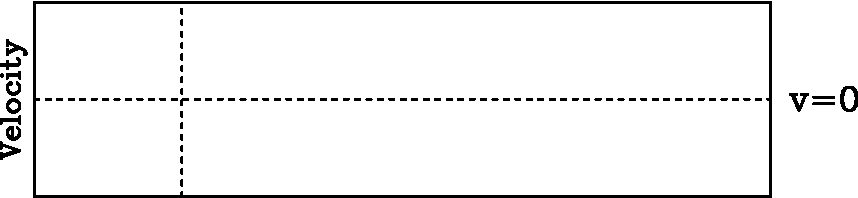
\includegraphics[width=0.85\textwidth]{vvst-plain-crop.pdf}\\
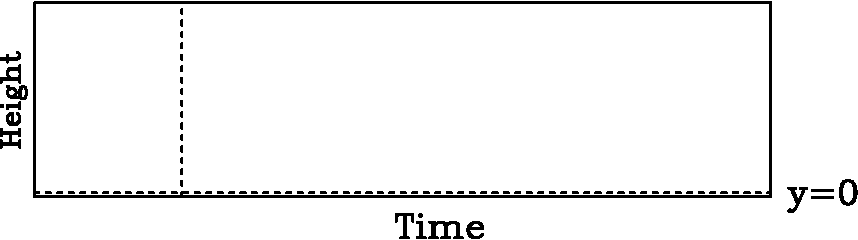
\includegraphics[width=0.85\textwidth]{xvst-plain-crop.pdf}
\end{center}
\end{minipage}

\newpage
Since the rocket's acceleration changes in flight, you can't use the constant-acceleration kinematics
formulae we've learned to understand the whole flight at once. However, the acceleration {\it is} piecewise constant.

This means that {\it one} copy of the constant-acceleration kinematics relations won't get the job done, but {\it two} 
copies will.

In problems like these, take the following approach:

\BI
\item Write down one set of kinematics relations (velocity and position) for the phase of the motion while the motor is on. Here, your time variable should represent the time since the rocket was launched. 
\item Write down a second set of kinematics relations for the phase of the motion while the motor is off, and the rocket is only moving under the influence of gravity. Here, your time variable represents the time since the motor turned off, since that is when this set of kinematics relations became valid.
\item Use the first set of kinematics relations to solve for the position and velocity at burnout. (Call this $y_b$ and $v_b$, or whatever other variables you want.) These values will become the initial position and velocity for the second phase. 
\item Solve for whatever you want to know about the second phase.
\EI

Answer the following. Ideally, figure out your answers in terms of $\tau$ (the rocket burn time), $g$, and $a_r$. You don't 
even have to plug numbers in if you don't want to!

\begin{enumerate}

\item How high above the ground is the rocket once its motor burns out? (Call this $y_b$.)
\vspace{2in}
\newpage
\item How fast is the rocket traveling once its motor burns out? (Call this $v_b$.)

\vspace{1.7in}
\item How fast is the rocket traveling when it reaches its maximum height?

\vspace{1.7in}
\item What is that maximum height?

\vspace{1.6in}
\item How long does it take for the rocket to land back on the ground?

\vspace{1.6in}
\end{enumerate}

\end{document}
